%%%%%%%%%%%%%%%%%%%%%%% file template.tex %%%%%%%%%%%%%%%%%%%%%%%%%
%
% This is a template file for Web of Conferences Journal
%
% Copy it to a new file with a new name and use it as the basis
% for your article
%
%%%%%%%%%%%%%%%%%%%%%%%%%% EDP Science %%%%%%%%%%%%%%%%%%%%%%%%%%%%

%\documentclass{webofc}
% option "twocolumn" for typesetting an article in two columns format (default one column)
 \documentclass[twocolumn]{webofc}
\usepackage{makecell}
\usepackage{upgreek}
\usepackage[varg]{txfonts}   % Web of Conferences font
\usepackage{hyperref}
\usepackage{url}

%% custom commands for thick lines in table
\makeatletter
\newcommand{\thickhlineTwo}{%
    \noalign {\ifnum 0=`}\fi \hrule height 2pt
    \futurelet \reserved@a \@xhline
}
\newcolumntype{"}{@{\hskip\tabcolsep\vrule width 1pt\hskip\tabcolsep}}
\makeatother

\makeatletter
\newcommand{\thickhlineOne}{%
    \noalign {\ifnum 0=`}\fi \hrule height 1pt
    \futurelet \reserved@a \@xhline
}
\makeatother

%%%%%%%%%%%%%%%%%%%%%%%%%%%%%%%%%%%%%%%%%%%%%%%%%%%%%%%%%%%%%%%%%%%%%%%%%%%%%
\hypersetup{colorlinks=true,citecolor=blue,urlcolor=blue,linkcolor=blue}
%%%%%%%%%%%%%%%%%%%%%%%%%%%%%%%%%%%%%%%%%%%%%%%%%%%%%%%%%%%%%%%%%%%%%%%%%%%%%
%
% Put here some packages required or/and some personnal commands
%
%
\begin{document}
%
\title{Overview of the front-end electronics of CMS HGCal - including readout and powering}
%
% subtitle is optionnal
%
%%%\subtitle{Do you have a subtitle?\\ If so, write it here}


\author{\firstname{Aidan} \lastname{Grummer}\inst{1}\fnsep\thanks{\email{aidan.grummer@cern.ch}} on behalf of the CMS Collaboration
        % \firstname{Isabelle} \lastname{Houlbert}\inst{2}\fnsep\thanks{\email{Mail address for second
        %      author if necessary}} \and
        % \firstname{blah} \lastname{Henri}\inst{3}\fnsep\thanks{\email{Mail address for last
        %      author if necessary}}
        % etc.
}

\institute{Fermi National Accelerator Lab.}


\abstract{
The end-cap calorimeters of CMS will be upgraded to a single High Granularity Calorimeter (HGCal) for the HL-LHC, including both silicon sensors and scintillator tiles with on-tile SiPMs as active elements. The readout of the active elements is performed by an ASIC (HGCROC in 130~nm CMOS technology) that measures the amplitude and arrival time of the signals. The amplitude is measured over a large dynamic range to allow calibration with single particles and the measurement of TeV showers. The time of arrival of high-energy showers will be measured with a precision of around 30 ps. A second pair of ``concentrator'' ASICs - ECON-T and ECON-D - takes the data from the HGCROC channels and packages them for transmission via optical links to the off-detector electronics. The ECON-T transmits trigger data at 40 MHz, to form part of the level-1 trigger. The ECON-D transmits concentrated data packets at up to 1 MHz, upon reception of a level-1 trigger signal. In addition to these ASICs, HGCal will use modified versions of common HL-LHC electronics developments, for the power chain and the optical control and readout. The dense nature of the HGCal provides additional challenges for the electronic boards and cabling. In this proceedings the overall HGCal front electronics scheme, including the latest performance of the HGCROC and ECON ASICs is presented.
}
%
\maketitle
%
\section{Introduction}
\label{intro}
Motivation for the HGCal upgrade of the CMS detector, for operation in HL-LHC, along with component details and science objectives may be found in~\cite{CMS:HGCalTDR}.
This proceedings provides an overview of the HGCal front-end. The front-end electronics are used to (1) digitize the signal from the sensors with the HGCal Readout Chip (HGCROC), (2) perform data concentration with the E-link Concentrators (ECON) and (3) to transmit the data using the low power gigabit transceiver (lpGBT) and electrical to optical conversion (VTRX+). Strategies for providing power and services to the front-end and composite systems testing will also be covered.

The main objective of the front-end is to deliver fundamental information needed for the calorimetry from the particle sensor to off detector electronics. The aim is to measure the charge over a large dynamic range: 0.2 fC — 10 pC. This range allows the calorimeter to make measurements of single minimum ionizing particles - used for calibration - as well as measurements of high energy (TeV level) jets. To mitigate the high pileup conditions expected from HL-LHC, it also needs to measure the time when a particle appears in the detector. Fine positional precision over a large area is needed for high quality jet resolution, and the detector is foreseen to have over 6 million readout channels.

The analogue pulse that appears when a particle is incident on a sensor is used to measure the charge the particle deposits and the time when the particle arrived. The shape of such a pulse is illustrated in figure~\ref{fig:pulse}. The digitization process is performed for several properties of this pulse. The charge is measured by reading out the analogue-to-digital pulse (ADC) directly for small charge deposits (small pulses). The time-over-threshold (TOT) is used for measuring large charge deposits (large pulses). The time of arrival of a signal (TOA) can also be measured at a given threshold depicted in the pulse diagram.

\begin{figure}[ht!]
\centering
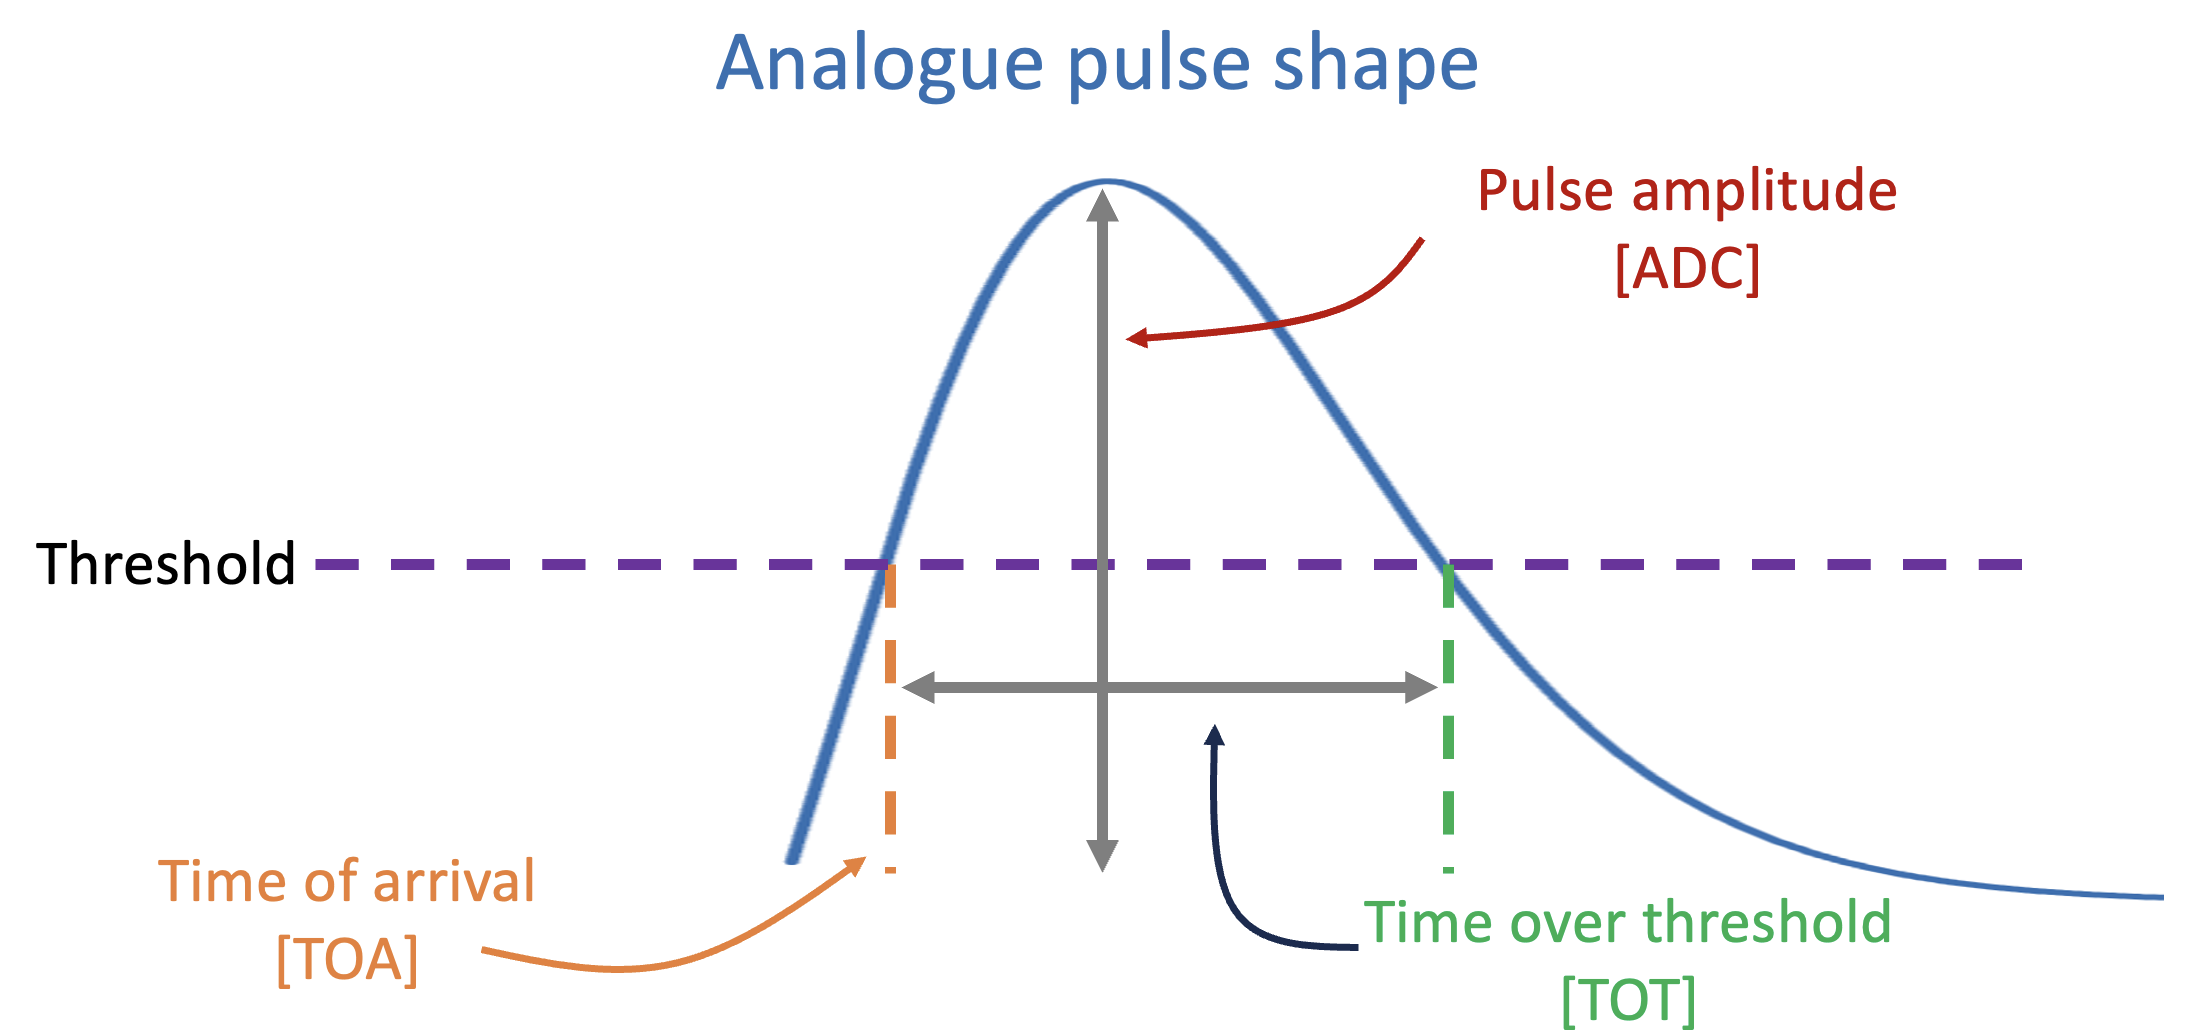
\includegraphics[height=4cm]{figures/PulseShape.png}
\caption{Diagram of the analogue pulse resulting from a particle incident on a single channel of the HGCal detector. Simplified definitions of the digitized quantities ADC, TOT and TOA are illustrated.}
\label{fig:pulse}
\vspace*{-1cm}
\end{figure}

\begin{table*}[htb!]
\caption{Front-end electronics constraints, introduced by the radiation environment, physical space availability, and capabilities necessary for broad science impact.}
\label{tab:req}
\centering
    \begin{tabular}{l|l} \hline
         Parameter & Specification\\ \thickhlineTwo
         Total ionizing dose&  200 Mrad\\ \hline

         \makecell[l]{Tolerance to single event effects (SEE) \\(average detector fluence)} &  Hadron fluence (E $>$ 20 MeV): 1$\times10^{14}$ cm$^{-2}$\\ \thickhlineOne

         Charge measurements with large dynamic range &  0.2 fC — 10 pC\\ \hline

         Time resolution &  25 ps\\ \hline

         Fit in limited physical space&  $\sim$5 mm gap\\ \hline
         \makecell[l]{Low power consumption\\(including digitization and concentration on \\DAQ and trigger paths)} & \makecell[l]{$\leq$ 20 mW/ch }\\ \hline

        \makecell[l]{Allow transfer of large data volumes required \\for good trigger and physics performance.} & \makecell[l]{Trigger path: $\sim$60 Tb/s \\DAQ path: $\sim$40 Tb/s}\\\hline
    \end{tabular}
\end{table*}

\begin{figure*}[ht!]
\centering
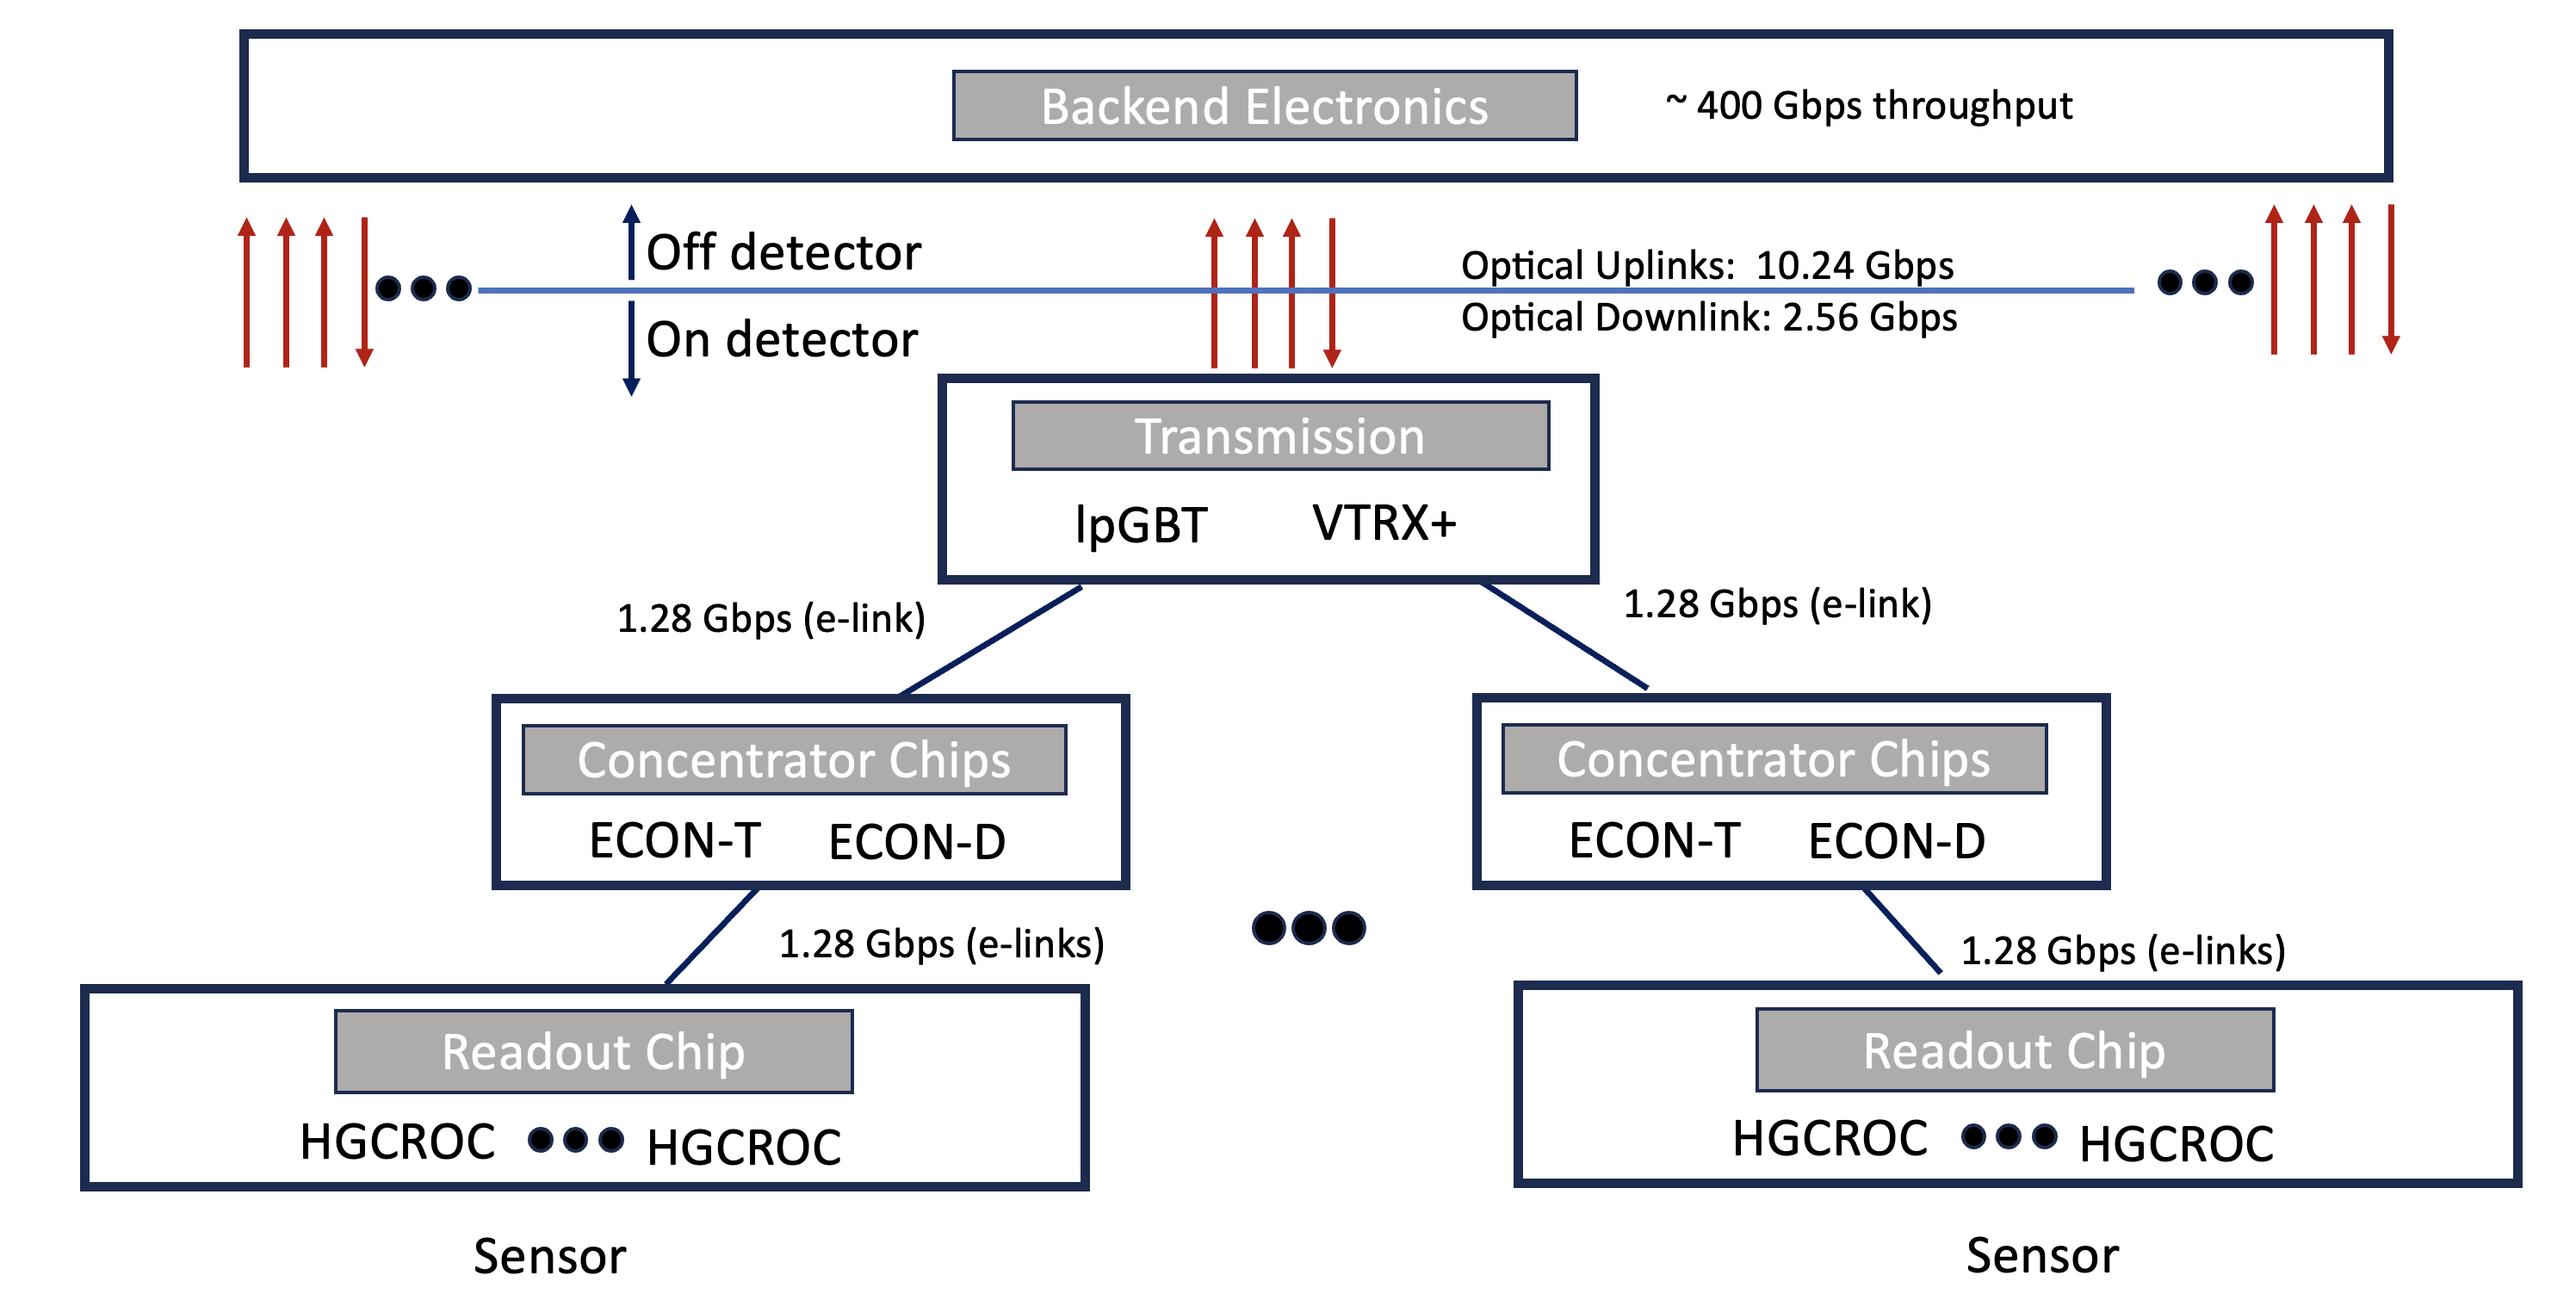
\includegraphics[height=8cm]{figures/ReadoutDiagram.png}
\caption{Illustration of the data path for the front-end readout. Each ASIC chip along the data path between the sensors and off detector backend electronics provides a unique role.}
\label{fig:diag}
\vspace*{-0.6cm}
\end{figure*}

\begin{figure*}[ht]
\centering
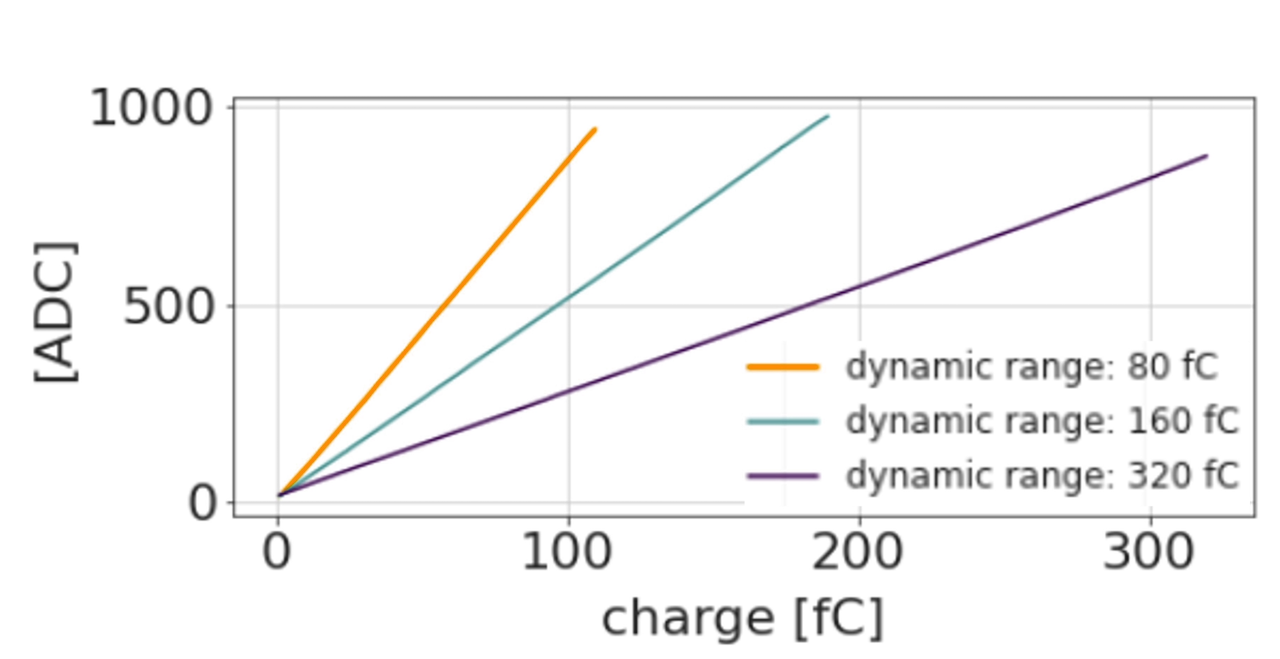
\includegraphics[width=6cm]{figures/roc-ADClinearity.png}
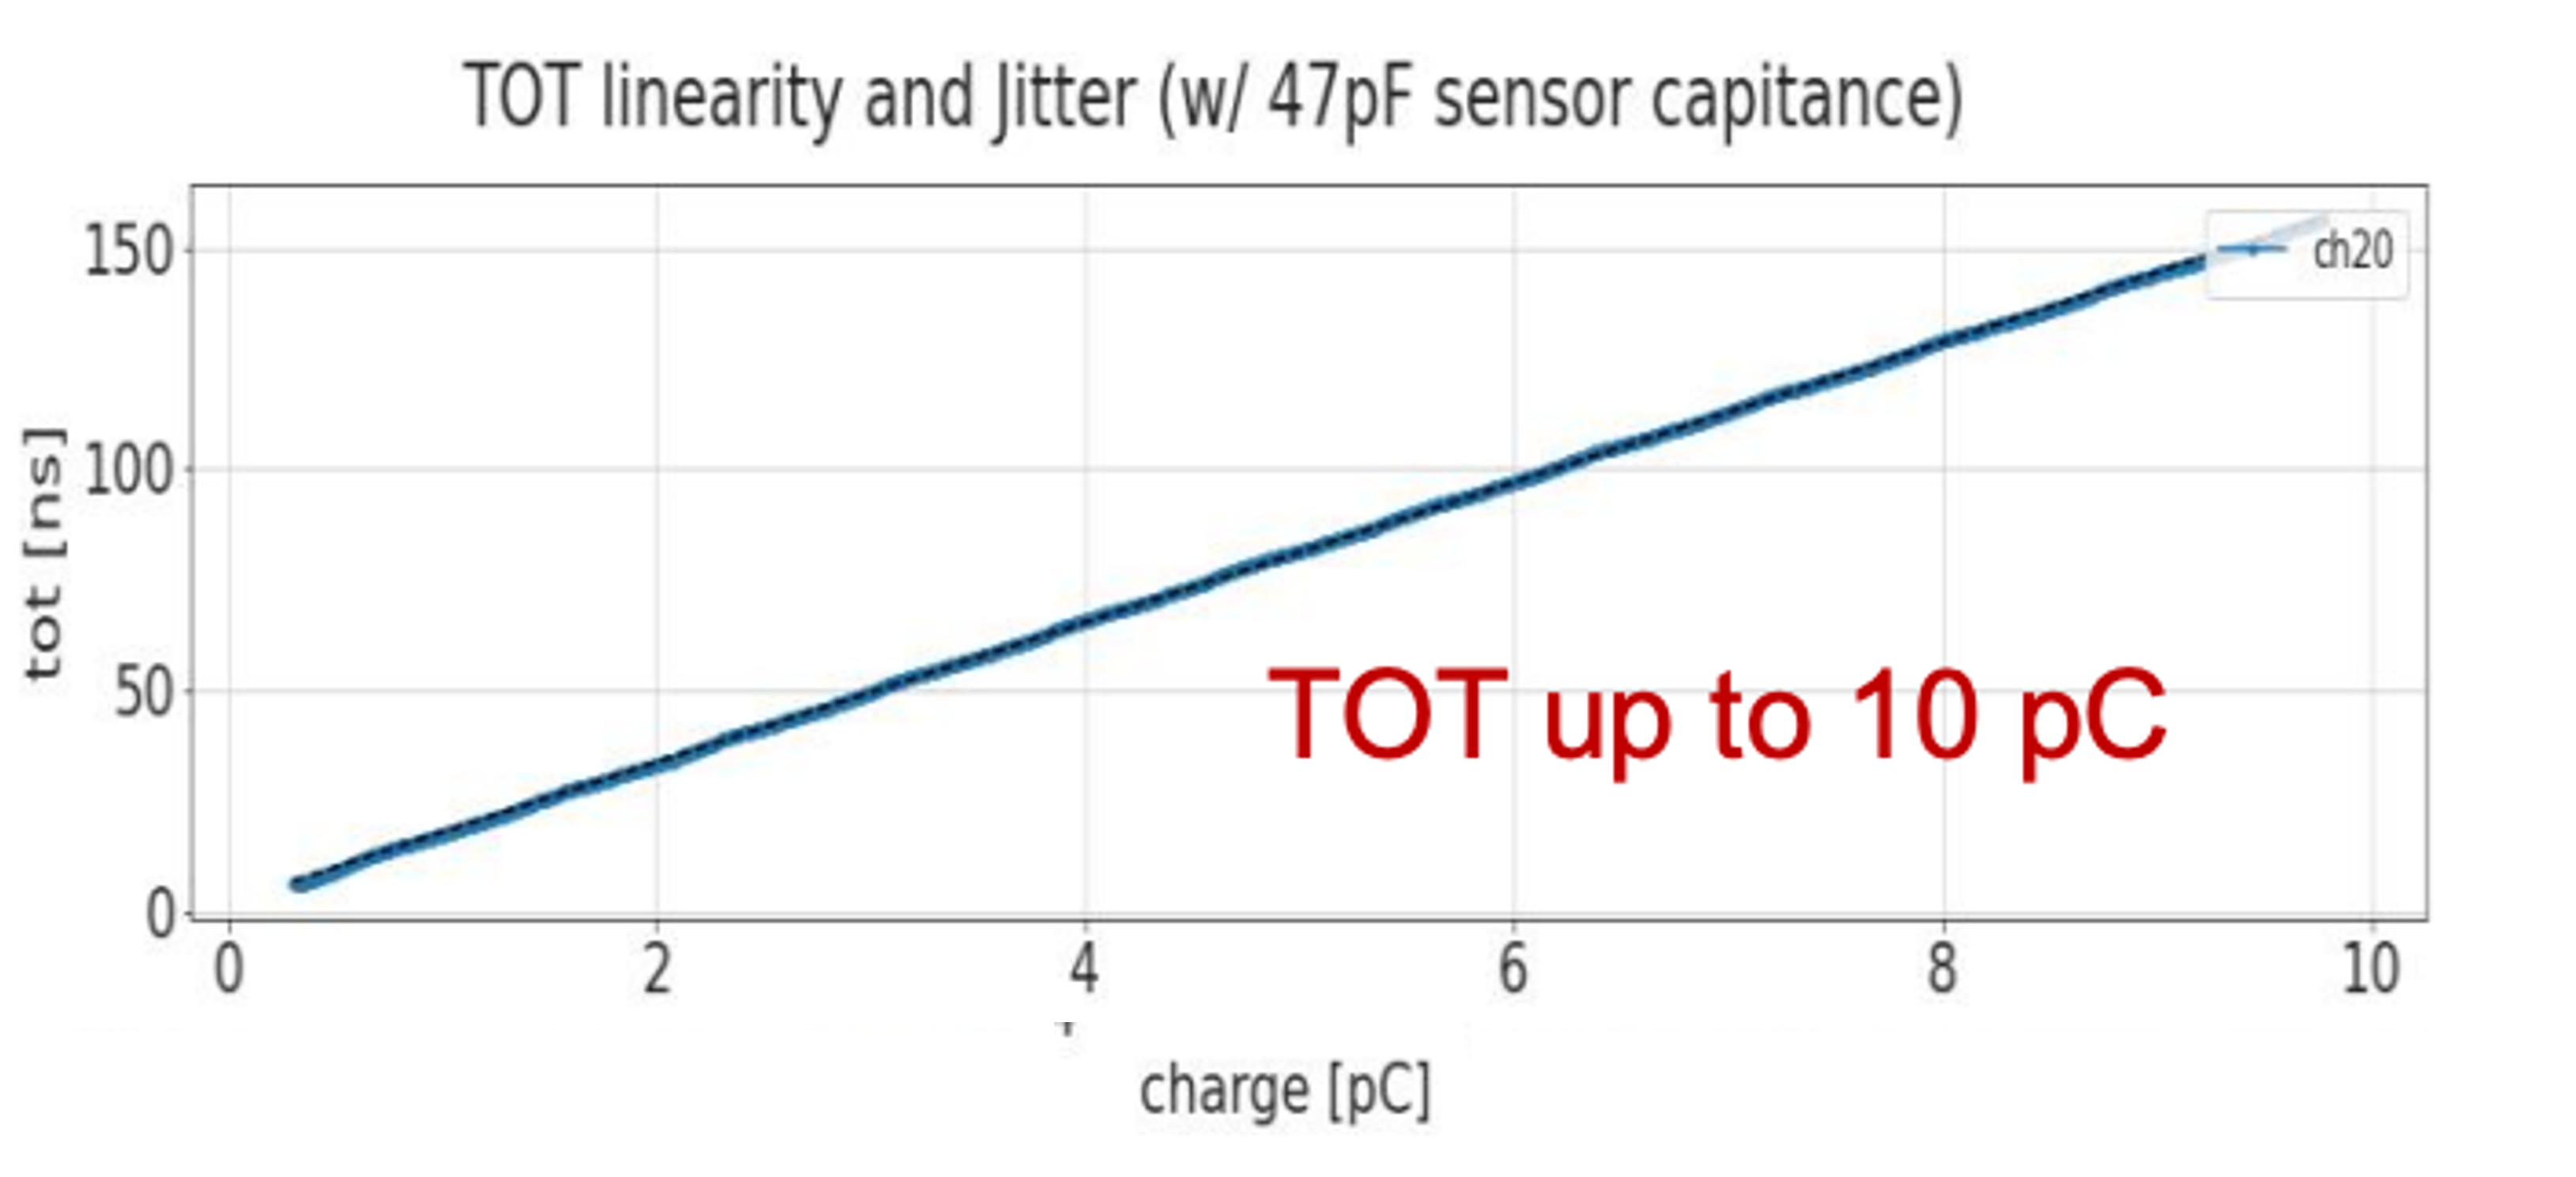
\includegraphics[width=7cm]{figures/roc-TOTlinearity.png}\\
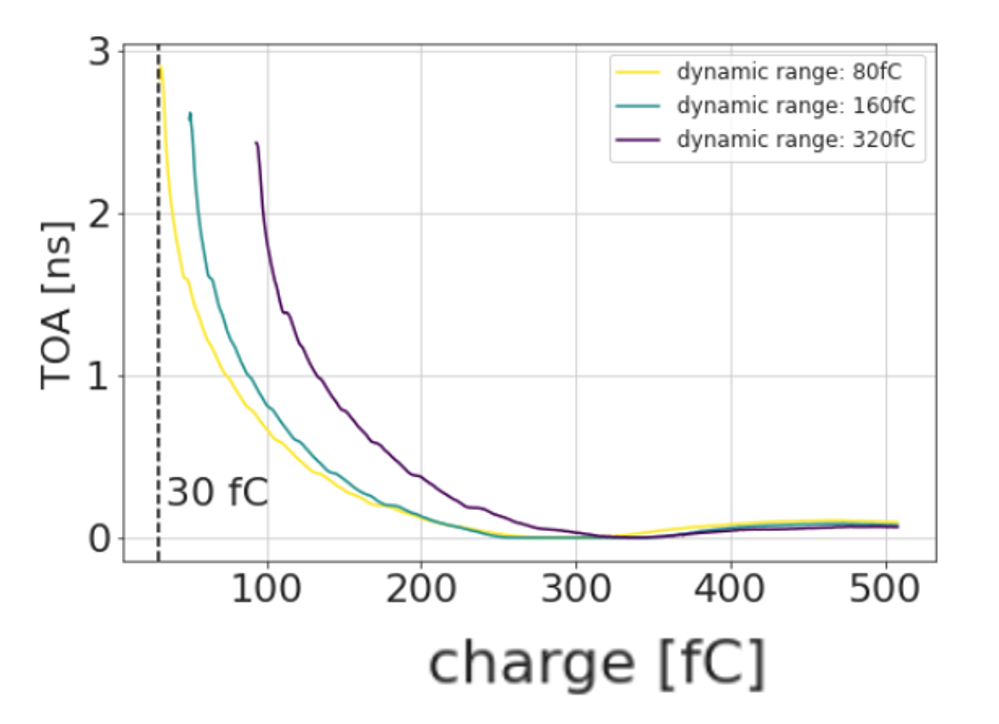
\includegraphics[width=6cm]{figures/roc-toaTimewalk.png}
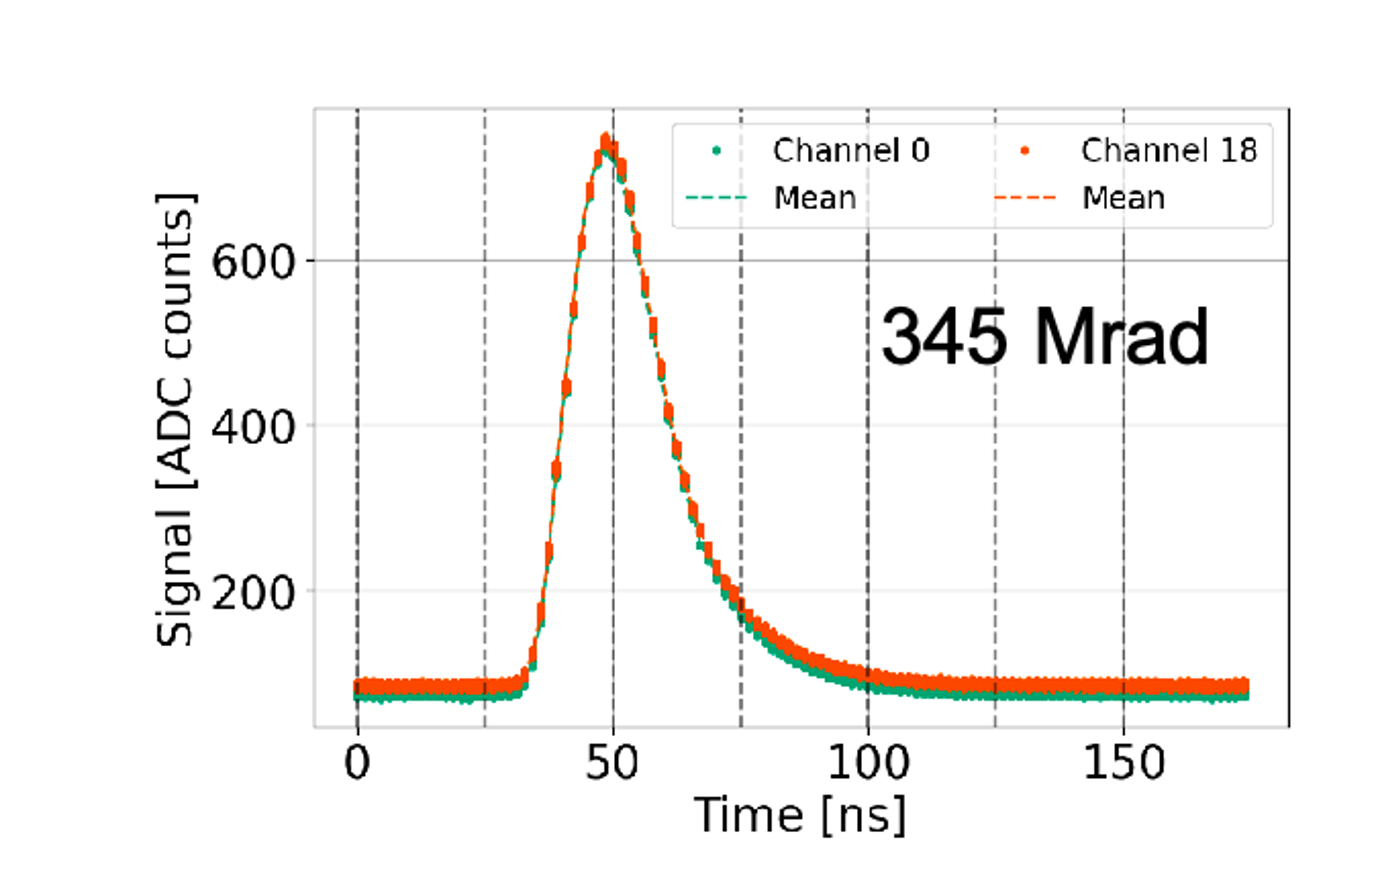
\includegraphics[width=8cm]{figures/roc-ADCirradiation.png}
\caption{(Top left plot) linearity of the HGCROC analogue to digital conversion (ADC) measured for different preamplifier gains is within specification, +/- 0.5\%. (Top right plot) the time over threshold (TOT) linearity is within specification, +/- 0.5\%. (Bottom left plot) time of arrival (TOA) as a function of charge shows a 2.5~ns time walk. (Bottom right plot) HGCROC ADC signal peak after 345 Mrad TID continues to show stable results.}
\label{fig:roc}
\vspace*{-0.6cm}
\end{figure*}

\begin{figure*}[ht]
\centering
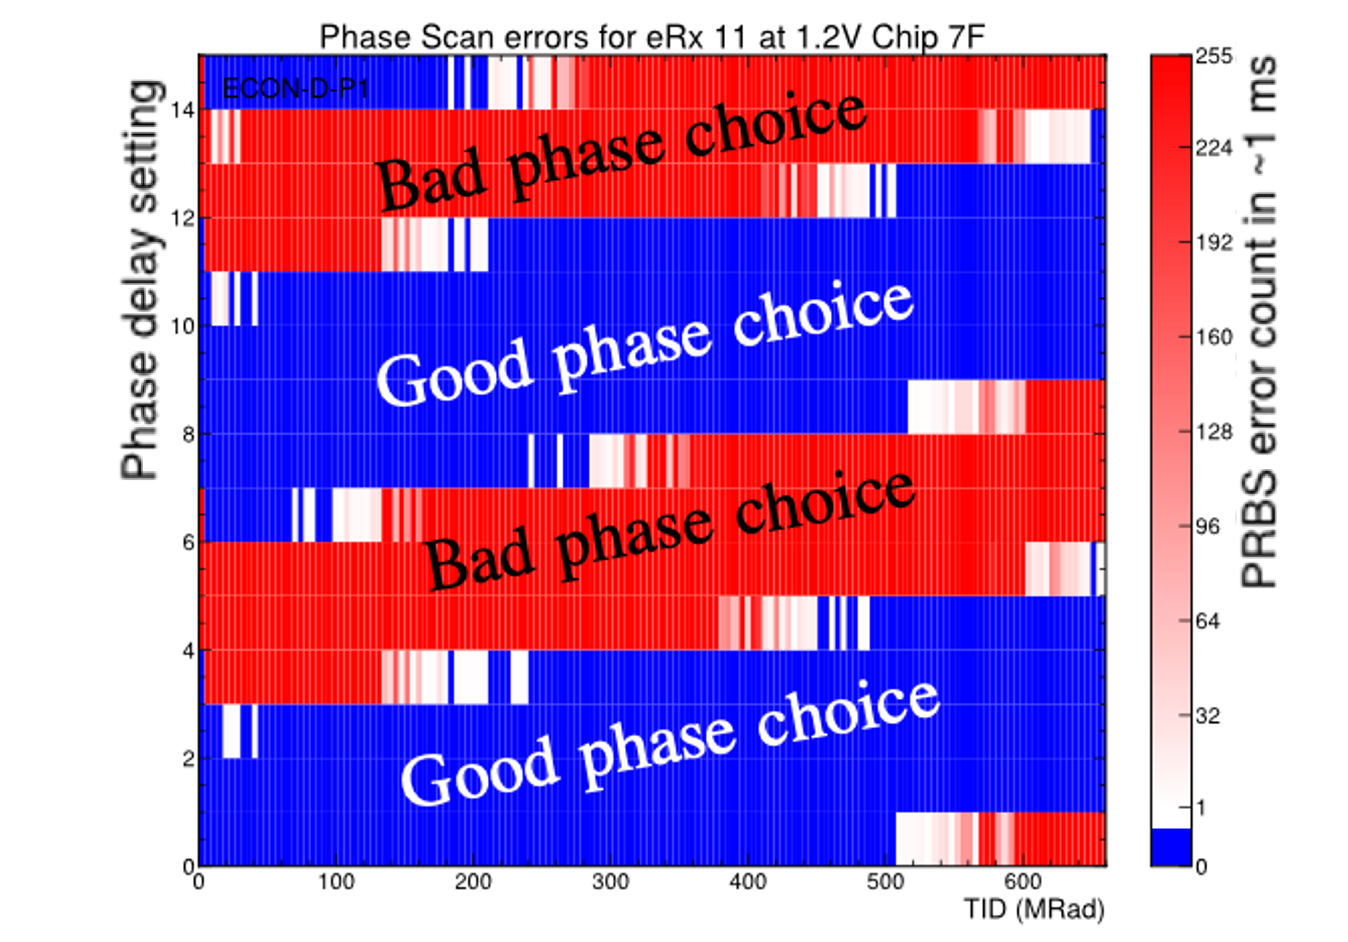
\includegraphics[height=5cm]{figures/econ-phaseTID.png}
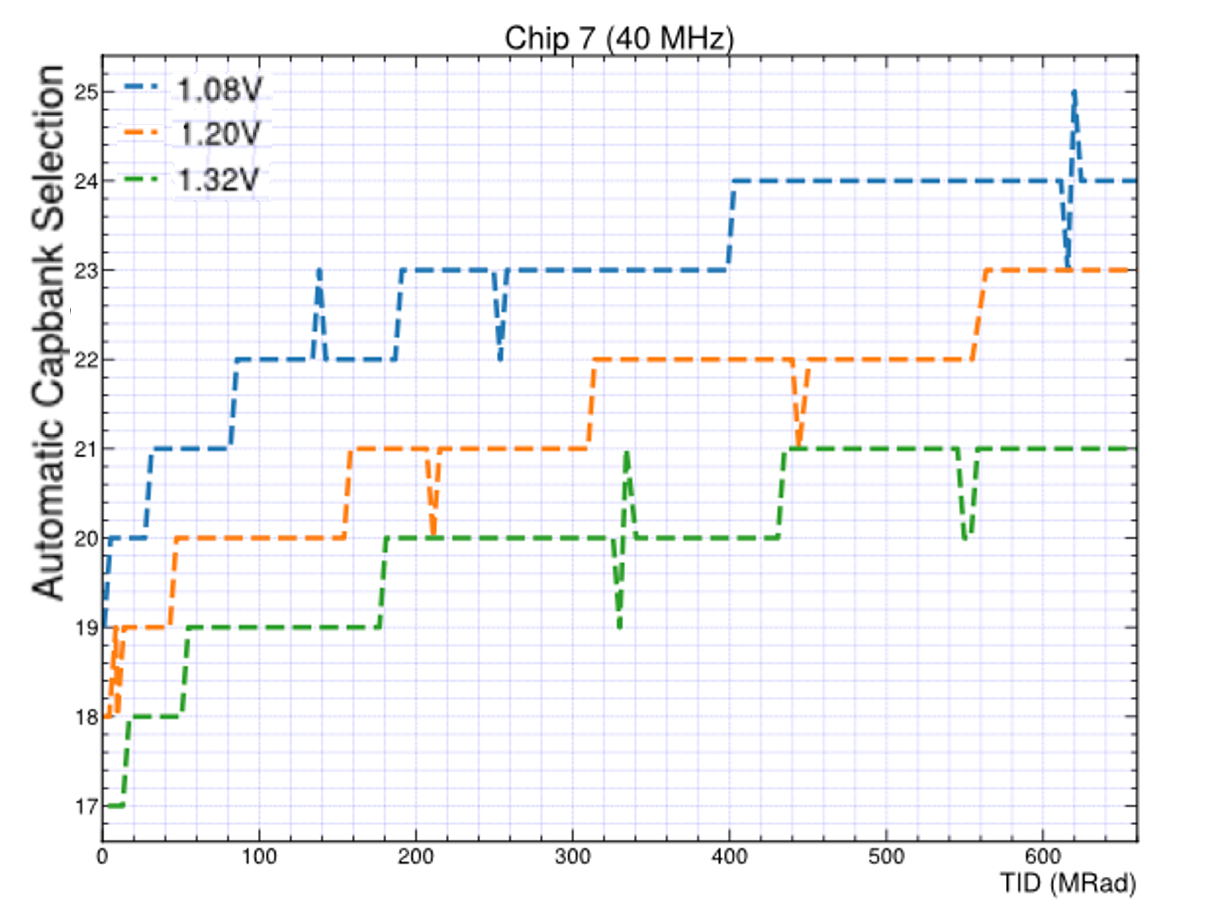
\includegraphics[height=5cm]{figures/econ-capPLLTID.png}
\caption{Total ionizing dose (TID) results for ECON ASICs. (Left plot) evidence of a shift of the good phase window at high TID. For a given choice of phase, the error rate is measured using a pseudo random bit stream; results are as expected. (Right plot) automatic capacitance selection for the phase lock loop (PLL) as a function of TID. Results are shown for the chip operated with different voltages. The capacitance selection results are as expected.}
\label{fig:econ}
\vspace*{-0.6cm}
\end{figure*}

\begin{figure}[ht]
\centering
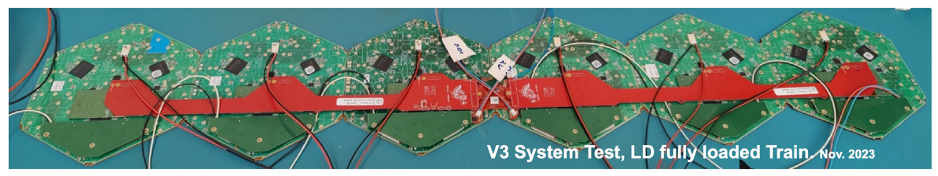
\includegraphics[width=8cm,clip]{figures/SixModules.png}
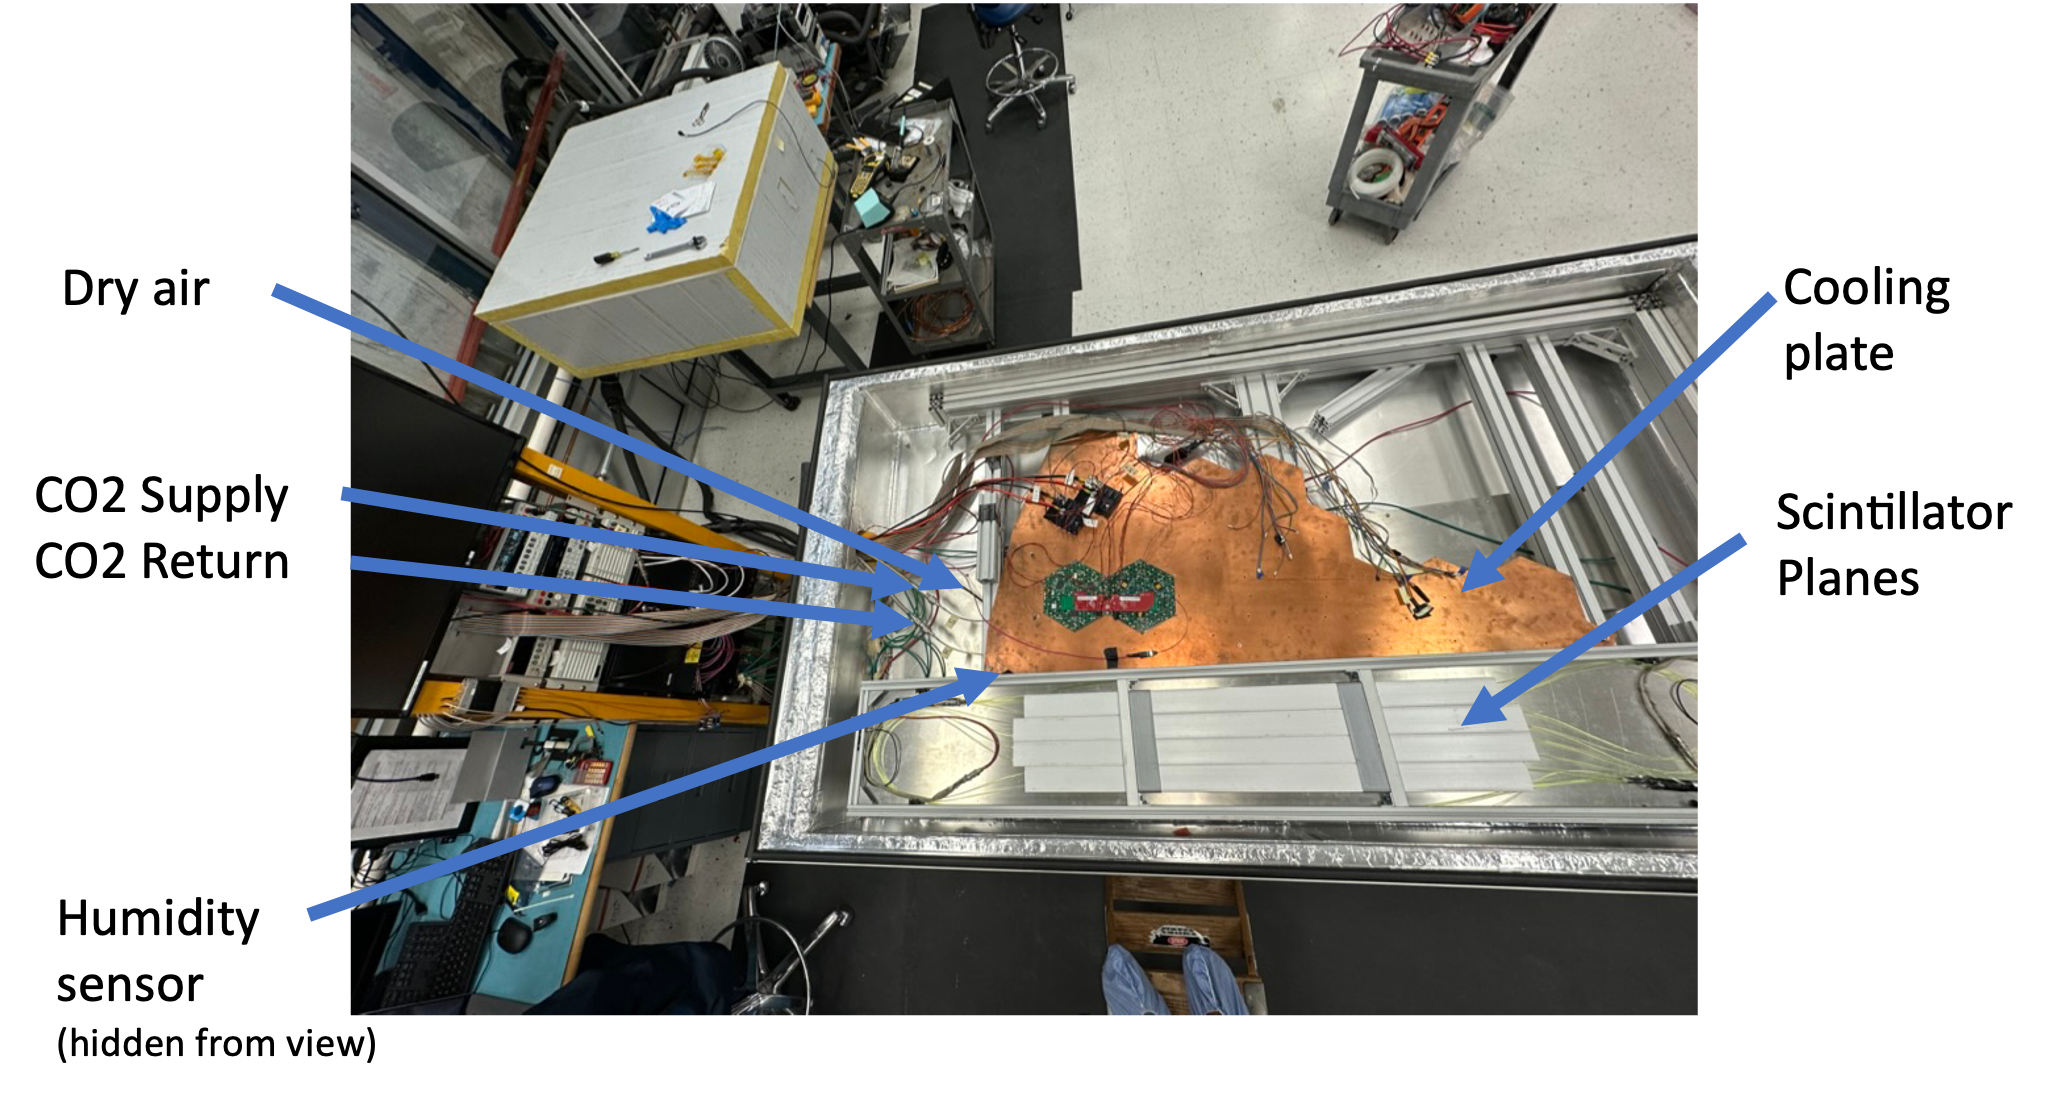
\includegraphics[width=8cm,clip]{figures/CoolingPlate.png}
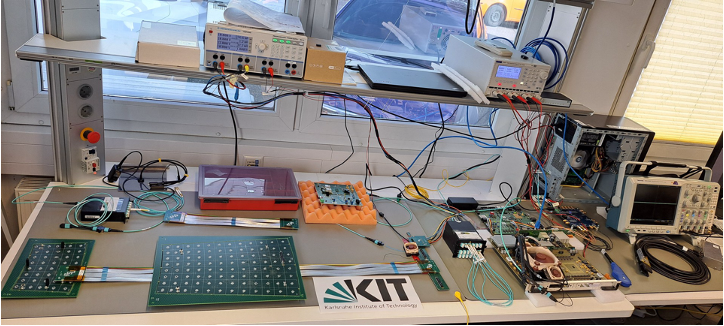
\includegraphics[width=7cm,clip]{figures/Scint.png}
    \caption{System test setups for (top picture) six low density silicon modules connected to an engine located at CERN, (middle picture) a two module silicon system in a cold test facility located at FNAL, (bottom picture) a two scintillator tileboard system located KIT. These systems allow testing of the operability of the front-end electronics in on detector conditions.}
\label{fig:systems}
\vspace*{-0.5cm}
\end{figure}


\section{Detector Requirements}
\label{sec:det_req}

The purpose of the front-end electronics, as noted above, is to digitize, concentrate, and transmit data off detector. Further requirements of the front-end are needed to fulfill this mandate. It is responsible for distributing a clock (provided from off-detector components) so that event data can be synchronized. The front-end must receive control signals in order set the detector configurations, for various modes of operation, and perform detector resets and re-syncs. It also needs to provide detector monitoring for characteristic data such as temperature, current, and voltage levels of detector components.

Requirements of the front-end design and operation imposed by environmental constraints, physical space and science objectives are summarized in table~\ref{tab:req}.

Additional challenges are introduced because almost every layer of the calorimeter has a different radius. This introduces complications in geometry of modules and connectors. A large variety in connector shapes are necessary in order to read out every module. Grouping modules allows for a uniform scheme to read out data.

\section{Readout scheme}
\label{sec:readout}

A diagram of the data readout scheme is show in figure~\ref{fig:diag}. The HGCROC reads out data at 1.28~GHz, the ECON concentrates the data and passes it on to the lpGBT at 1.28~GHz. The lpGBT, together with the VTRX+, serializes the data and converts the electrical signal to optical signal in order to transmit it to off detector electronics at 10.24~GHz.

\subsection{Readout ASIC: HGCROC}
\label{sec:roc}
The HGCROC measures up to 72 readout channels on a module as well as 4 common mode channels to mitigate noise and 2 calibration channels.
Two separate data paths are generated by the chip: the trigger path and DAQ path.
The trigger path provides a sum of 4 or 9 channels, depending on the type of module it is reading out, and provides a 7-bit floating point number. The trigger path outputs four 1.28~Gbps links. The DAQ path contains a DRAM with a depth of 512, a circular buffer, and can store the full event info (ADC, TOT and TOA) for 12.5~$\upmu$s. The DAQ path outputs two 1.28~Gbps output links. The HGCROC uses I2C protocol for slow control, uses a 320~MHz clock, and is capable of receiving fast commands, used, for example, for chip resets.

Characterization of the HGCROC is well advanced. The linearity of the full ADC range is within +/- 0.5 \%, meeting the design specification and allowing for good calibration of the detector. The TOT range linearity is also within a range +/- 0.5 \%, the jitter around 25~ps and the TOA measurements shows a 2.5~ns time walk. These are all within specifications of the chip design. The ADC and TOT linearity measurements and the TOA time walk data are shown in figure~\ref{fig:roc}.

Several radiation campaigns to investigate the behavior of the HGCROC have been completed. Total ionizing dose (TID) results demonstrated that at 5~$^{\circ}$C the chip behavior is very stable up to 350~Mrad  with almost no changes in the ADC, the time to digital conversions (TDC), or the phase lock loop (PLL) behavior. The ADC pulse shape after the chip received 345~Mrad TID is shown in figure~\ref{fig:roc}. HGCal module and detector system tests operated with the HGCROC are continuing. Pre-production HGCROC chips were received at end of February 2024.

\subsection{Data concentration: ECON chips}
\label{sec:econ}
The ECON chips concentrate data to reduce the number of data links in the path. They also provide utilities to monitor the synchronization between the HGCROC and ECON, and report this information upstream.

Two versions of ECON are designed to operate in the trigger path and the DAQ path. ECON-T is used for the trigger path. Its roll is to select or compress HGCROC trigger data for transmission off detector at 40 MHz. The ECON-T can be configured with I2C slow control commands to compress data with one of four algorithms: Threshold-sum, Best-Choice, Super trigger cell, Auto-encoder (“AI on Chip”). The ECON-D is used for the DAQ path. It performs digital processing of sensor data for events passing L1 trigger up to 1 MHz (nominal operation expected at 750 kHz). ECON-D applies zero-suppression to avoid readout of channel data that does not have a pulse above the nominal noise and performs alignment of channels from multiple HGCROCs.

Radiation campaigns have been used to demonstrate the ECON chips maintain excellent performance in harsh radiation environments. No single event upsets have been observed in slow control I2C registers. The campaigns were used to set upper limits on the cross section of errors requiring a reset. Good behavior was observed up to 660 Mrad when the chip is operated at 1.2V. The test facility used for TID testing was the CERN ObeliX X-ray. There was evidence of a small error rate at >450 Mrad for ECON-D-P1 when operated at the lowest voltage, 1.08~V. This is well within the HGCal design requirements of 200 Mrad. Operability of the ECON during TID testing is demonstrated in figure~\ref{fig:econ}, showing the expected change in the optimal phase and capacitance settings with exposure to higher levels of TID.

The ECON engineering run is complete and the project will receive 24 thousand ECONs shortly after the conference date. The amount is about half of the total number needed for the detector. Characterization and testing will happen the summer 2024. All ECONs are expected to be produced and tested by early 2025.

\subsection{Data transmission: Engines}
\label{sec:eng}

The ``engine'' components of the HGCal detector are custom designed PCB boards that utilize the CERN designed lpGBT ASIC together with the CERN VTRX+ ASIC to transmit data off detector through optical fibers. The engines serialize data from the up to 7 concentrator chips. Uplinks send data at 10.24~Gbps. Low density (LD) engines supports up to 6 full LD silicon modules. High density (HD) engines support up to 3 full HD silicon modules. The engines are connected to the modules with passive PCBs that have many variants (>50) to accommodate the complicated geometries of the detector layers and small envelope between layers.

\section{Front-end powering: DC-to-DC converters}
\label{sec:power}

A single low voltage power level will be provided to the detector. Custom DC-to-DC converters are used to step the voltage down to appropriate levels for operating the modules. Custom coils and shields are used to avoid introducing noise into the readout. BusBars will be used to distribute power throughout the system. The BusBars are Heavy-copper flex PCBs and provide tight coupling between supply and returns. This method of power distribution is intrinsically radiation tolerant (utilizing polyimide-based insulation).

\section{A suite of test systems}
\label{sec:systems}

A rigorous set of test systems and facilities are setup at sites around the world. Some of the setups may be seen in figure~\ref{fig:systems}.
The system tests ensure robust performance of the entire HGCal system (including the front-end electronics) from prototypes through pre-production and full production.

\section{Conclusions}
\label{sec:conclusion}
No project show-stoppers have been found in any part of the system, despite challenging custom ASICs and extreme radiation tolerance constraints.
The HGCROC preproduction chips are becoming available now (up to 5\% of detector) and the production chips are expected by the end of 2024. The ECON engineering run chips will arrive soon after the conference date. All ECON chips will be produced and tested by early 2025.
More test beams are expected in the near future for system testing (including in a magnetic field) and ASIC radiation tolerance testing.
Cassette (detector unit comprised of tens of modules) pre-production is planned to begin at the end of the year.

Several other HGCal project topics were covered at the CALOR2024 conference including on mechanical challenges, backend electronics developments, and event reconstruction efforts.


% \section{Section title}
% \label{sec-1}
% For bibliography
% \subsection{Subsection title}
% \label{sec-2}
% Don't forget to give each section, subsection, subsubsection, and
% paragraph a unique label (see Sect.~\ref{sec-1}).
%
% For one-column wide figures use syntax of figure~\ref{fig-1}
% \begin{figure}[h]
% % Use the relevant command for your figure-insertion program
% % to insert the figure file.
% \centering
% 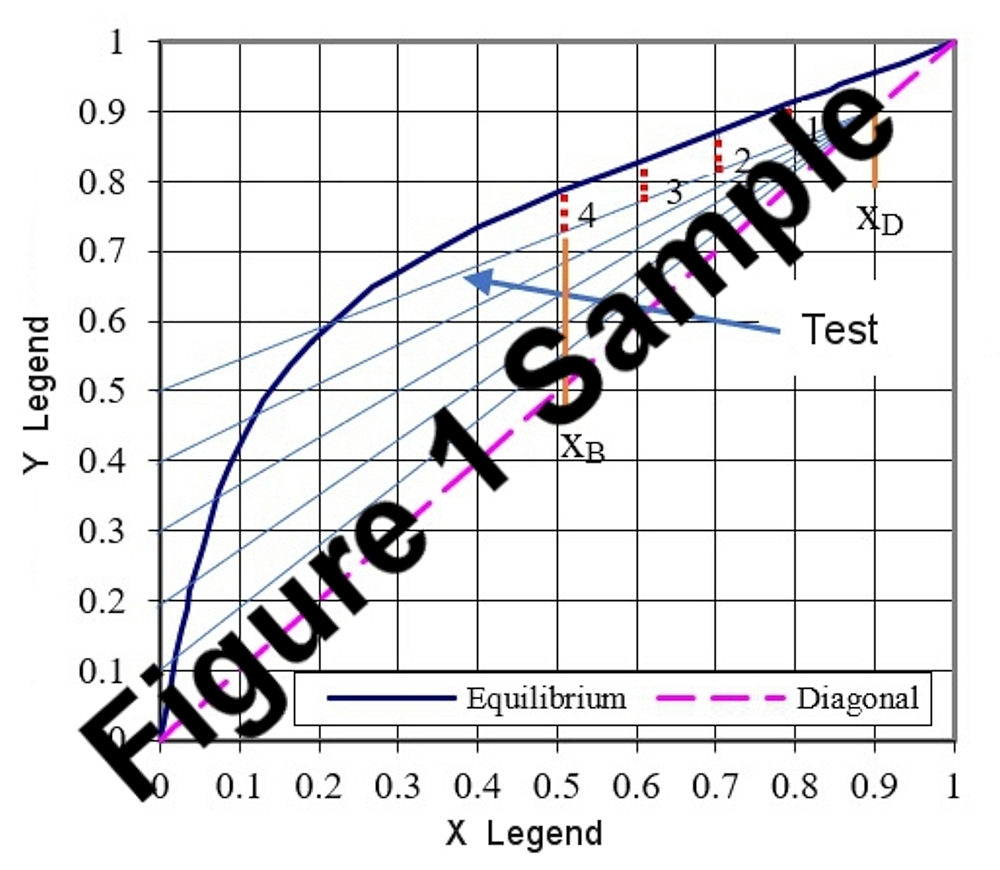
\includegraphics[width=5cm,clip]{fig-1-sample}
% \caption{Please write your figure caption here}
% \label{fig-1}       % Give a unique label
% \end{figure}
%
% For two-column wide figures use syntax of figure~\ref{fig-2}
% \begin{figure*}
% \centering
% % Use the relevant command for your figure-insertion program
% % to insert the figure file. See example above.
% % If not, use
% \vspace*{1cm}       % Give the correct figure height in cm
% 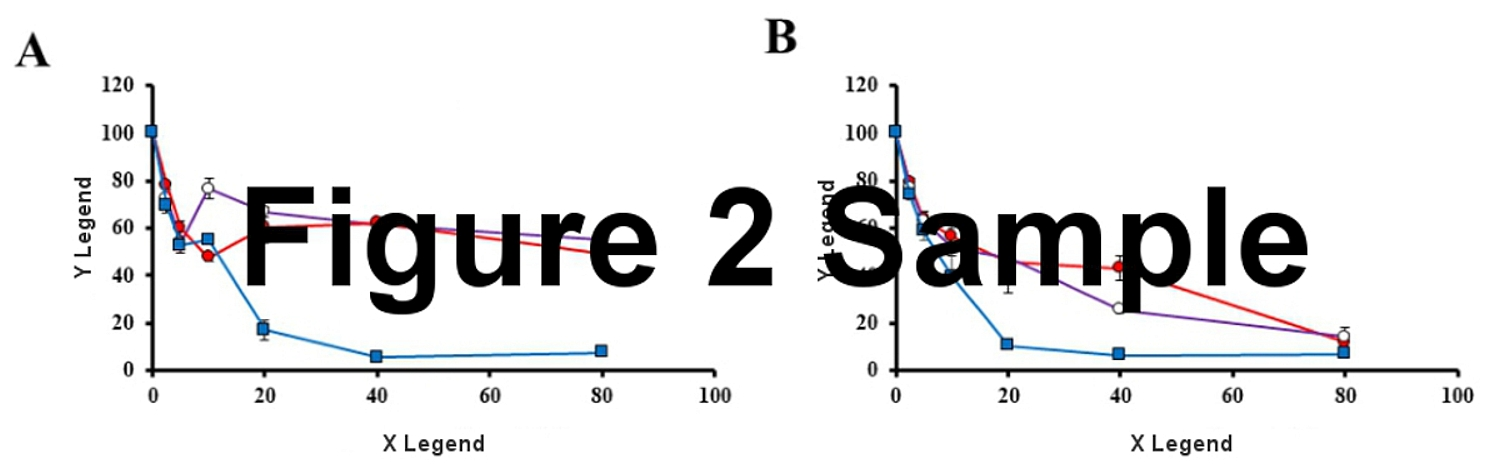
\includegraphics[width=8cm,clip]{fig-2-sample}
% \caption{Please write your figure caption here}
% \label{fig-2}       % Give a unique label
% \end{figure*}
%
% For tables use syntax in table~\ref{tab-1}.
% \begin{table}
% \centering
% \caption{Please write your table caption here}
% \label{tab-1}       % Give a unique label
% % For LaTeX tables you can use
% \begin{tabular}{lll}
% \hline
% first & second & third  \\\hline
% number & number & number \\
% number & number & number \\
% number & number & number \\\hline
% \end{tabular}
% % Or use
% \vspace*{5cm}  % with the correct table height
% \end{table}
%
% BibTeX or Biber users please use (the style is already called in the class, ensure that the "woc.bst" style is in your local directory)
\bibliography{src/proc.bib}
%
\end{document}

% end of file template.tex
